
\section{Overview of the proof strategy for $k \to \infty$}

\PvdH{References need to be included once Section 1 is updated.}

The proof of Theorem~\ref{thm:mainktoinfty} follows the same strategy as outlined in Section~\ref{sec:proof_outline} and executed in Section~\ref{sec:proofs_fixed_k}. However, the fact that $k = k_n \to \infty$ as $n \to \infty$, introduces additional technical challenges. For example, the coupling we use becomes less exact so that we can no longer use Lemma~\ref{lem:coupling_edges} to conclude that triangle counts in $\GPo$ and $\Gbox$ are asymptotically equivalent. In this section we explain the challenges with each step and give a detailed overview of the structure for the proof of Theorem~\ref{thm:mainktoinfty} using intermediate results for each of the steps. Since we are ultimately interested in recovering the scaling of $c(k_n;G_n)$, which Theorem~\ref{thm:mainktoinfty} claims is $\gamma(k_n)$, we need to show that each step only introduces error terms that are of smaller order, i.e. that are $\smallO{\gamma(k_n)}$. To this end we define the scaling function
\begin{equation}\label{eq:def_scaling_function}
	s(k) = \begin{cases}
		k^{-(4\alpha - 2)} &\mbox{if } \frac{1}{2} < \alpha < \frac{3}{4},\\
		\log(k) k^{-1} &\mbox{if } \alpha = \frac{3}{4},\\
		k^{-1} &\mbox{if } \alpha > \frac{3}{4},
	\end{cases}
\end{equation}
so that $\gamma(k) = \bigT{s(k)}$ as $k \to \infty$. We will end this section with the proof of Theorem~\ref{thm:mainktoinfty}, based on the intermediate results.

\begin{remark}[Diverging $k_n$]
Throughout the remainder of this paper $\{k_n\}_{n \ge 1}$ will always denote a sequence of integers satisfying $k_n \to \infty$ and $k_n = \smallO{n^{\frac{1}{2\alpha + 1}}}$, as $n \to \infty$.
\end{remark}

We start with introducing a slightly modified version of the local clustering function, which will be convenient for computations later,
\begin{equation}\label{eq:def_local_clustering_ast_general}
	c^\ast(k;G) = \frac{1}{\Exp{N_k}} \sum_{v \in V(G) \atop \text{deg}(v)=k} c(v).
\end{equation}
Notice that the only difference between $c(k;G)$ and $c^\ast(k;G)$ is that we replace $N_G(k)$ by its expectation $\Exp{N_G(k)}$. The advantage is that now, the only randomness is in triangle counting. In addition, note that since $\Exp{N_G(k)} > 0$ a case distinction for $N_k$ is no longer needed for $c^\ast(k;G)$. It is however still relevant since we are eventually interested in $c(k;G)$. Following the notational convention, throughout the remainder of this paper we write $c^\ast(k; \GPo)$ and $c^\ast(k; \Gbox)$ to denote the modified local clustering function in $\GPo$ and $G_{\mathcal{P},n}(\alpha,\nu)$, respectively.

Figure~\ref{fig:overview_proof} shows a schematic overview of the proof of Theorem~\ref{thm:mainktoinfty} based on the different propositions described below, plus the sections in which theses propositions are proved. Observe that the order in which the intermediate results are proved is reversed with respect to the natural order of reasoning. This does not create any circular logic, since each intermediate result is independent of the others. We choose this order because results proved in the later stages are helpful to deal with error terms coming up in proofs at earlier stages and hence help streamline those proofs. 

\begin{figure}[!t]
\centering

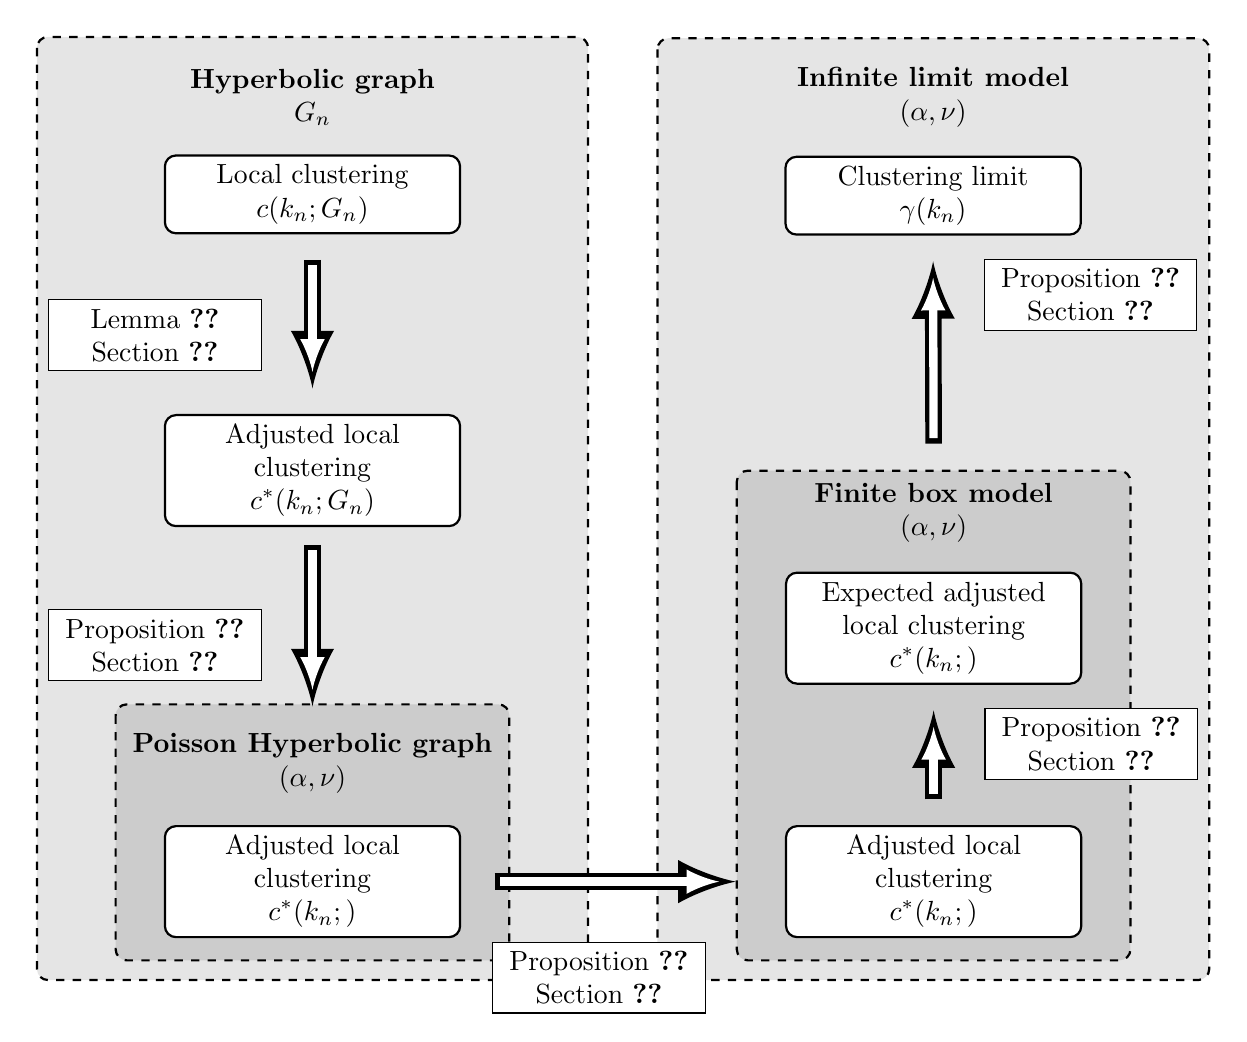
\begin{tikzpicture}

\pgfdeclarelayer{background}
\pgfdeclarelayer{foreground}
\pgfsetlayers{background,main,foreground}

\tikzstyle{block} = [draw, text centered, rounded corners, draw=black, thick, fill=white]
\tikzstyle{textblock} = [draw, text centered, draw=black, fill=white]

\tikzset{
  double arrow/.style args={#1 colored by #2 and #3}{
    -latex,line width=#1,#2, % first arrow
    postaction={draw,-latex,#3,line width=(#1)/2,
                shorten <=(#1)/3,shorten >=(#1)}, % second arrow
  }
}

\draw node (anchor) at (0,0) {};

%Hyperbolic graph: top left

\path (anchor)+(0,0) node (hyp_header) {\begin{minipage}[c]{10em}
	\begin{center}
		\textbf{Hyperbolic graph}\\
		$G_n$
	\end{center}
\end{minipage}};

\path (hyp_header.south)+(0,-0.75) node (c_hyp) [block] {\begin{minipage}[c]{10em}
	\begin{center}
	Local clustering\\
	$\displaystyle c(k_n;G_n)$
	\end{center}
\end{minipage}};






%Adjusted local clustering: middle left

\path (c_hyp.south)+(0,-3) node (c_ast_hyp) [block] {\begin{minipage}[c]{10em}
	\begin{center}
	Adjusted local clustering\\
	$\displaystyle c^\ast(k_n;G_n)$
	\end{center}
\end{minipage}};

\path (c_ast_hyp.north)+(-2,1) node (hyp_text) [textblock] {\begin{minipage}[c]{7em}
	\begin{center}
		Lemma \ref{lem:clustering_ast_H}\\
		Section~\ref{ssec:coupling_H_HP}
	\end{center}
\end{minipage}};

%Poisson Hyperbolic graph: middle left

%\path (c_hyp.south)+(0,-6) node (c_pois_hyp) [block] {\begin{minipage}[c]{12em}
%	\begin{center}
%	Local clustering\\
%	$\displaystyle c_{\widetilde{\H},n}(k_n)$
%	\end{center}
%\end{minipage}};



\path (c_ast_hyp.south)+(0,-3) node (pois_hyp_header) {\begin{minipage}[c]{13em}
	\begin{center}
		\textbf{Poisson Hyperbolic graph}\\
		$\GPo(\alpha,\nu)$
	\end{center}
\end{minipage}};

\path (pois_hyp_header.north)+(-2,1) node (pois_hyp_text) [textblock] {\begin{minipage}[c]{7em}
	\begin{center}
		Proposition \ref{prop:clustering_ast_H_Pois}\\
		Section~\ref{ssec:coupling_H_HP}
	\end{center}
\end{minipage}};





%Poisson Hyperbolic graph: bottom left

\path (pois_hyp_header.south)+(0,-1) node (c_ast_pois_hyp) [block] {\begin{minipage}[c]{10em}
	\begin{center}
	Adjusted local clustering\\
	$\displaystyle c^\ast(k_n; \GPo)$
	\end{center}
\end{minipage}};



%Infinite limit model: top right



\path (hyp_header.east)+(6,0) node (pois_header) {\begin{minipage}[c]{10em}
	\begin{center}
		\textbf{Infinite limit model}\\
		$\Ginf(\alpha, \nu)$
	\end{center}
\end{minipage}};

\path (pois_header)+(0,-1.25) node (c_infty) [block] {\begin{minipage}[c]{10em}
	\begin{center}
	Clustering limit\\
	$\displaystyle \gamma(k_n)$
	\end{center}
\end{minipage}};

\path (c_infty.south)+(2,-0.75) node (exp_c_pois_text) [textblock] {\begin{minipage}[c]{7em}
	\begin{center}
		Proposition \ref{prop:convergence_average_clustering_P_n}\\
		Section \ref{sec:clustering_Pn_to_P}
	\end{center}
\end{minipage}};




%Finite box model: bottom right

\path (c_ast_pois_hyp.east)+(6,0) node (c_ast_pois_n) [block] {\begin{minipage}[c]{10em}
	\begin{center}
	Adjusted local clustering\\
	$\displaystyle c^\ast(k_n; \Gbox)$
	\end{center}
\end{minipage}};

\path (c_ast_pois_n.south)+(-4.25,-0.5) node (c_ast_pois_n_text) [textblock] {\begin{minipage}[c]{7em}
	\begin{center}
		Proposition \ref{prop:couling_c_H_P}\\
		Section \ref{ssec:coupling_HP_ast_P}
	\end{center}
\end{minipage}};

\path (c_ast_pois_n.north)+(0,2.5) node (exp_c_pois_n) [block] {\begin{minipage}[c]{10em}
	\begin{center}
	Expected adjusted local clustering\\
	$\displaystyle \Exp{c^\ast(k_n; \Gbox)}$
	\end{center}
\end{minipage}};

\path (exp_c_pois_n.south)+(2,-0.75) node (exp_c_pois_n_text) [textblock] {\begin{minipage}[c]{7em}
	\begin{center}
		Proposition \ref{prop:concentration_local_clustering_P_n}\\
		Section \ref{sec:concentration_c_P_n}
	\end{center}
\end{minipage}};

\path (exp_c_pois_n.north)+(0,0.75) node (pois_n_header) {\begin{minipage}[c]{13em}
	\begin{center}
		\textbf{Finite box model}\\
		$\Gbox(\alpha, \nu)$
	\end{center}
\end{minipage}};








%Arrows

\path (c_hyp.south)+(0,-0.2) node (arrow_1l) {};
\path (c_ast_hyp.north)+(0,0.2) node (arrow_1r) {};

\draw [double arrow=6pt colored by black and white] (arrow_1l) -- (arrow_1r);

\path (c_ast_hyp.south)+(0,-0.1) node (arrow_2l) {};
\path (pois_hyp_header.north)+(0,0.1) node (arrow_2r) {};

\draw [double arrow=6pt colored by black and white] (arrow_2l) -- (arrow_2r);

\path (c_ast_pois_hyp.east)+(0.3,0) node (arrow_3l) {};
\path (c_ast_pois_n.west)+(-0.5,0) node (arrow_3r) {};

\draw [double arrow=6pt colored by black and white] (arrow_3l) -- (arrow_3r);

\path (c_ast_pois_n.north)+(0,0.2) node (arrow_4l) {};
\path (exp_c_pois_n.south)+(0,-0.2) node (arrow_4r) {};

\draw [double arrow=6pt colored by black and white] (arrow_4l) -- (arrow_4r);

\path (exp_c_pois_n.north)+(0,1.5) node (arrow_5l) {};
\path (c_infty.south)+(0,-0.2) node (arrow_5r) {};

\draw [double arrow=6pt colored by black and white] (arrow_5l) -- (arrow_5r);

\begin{pgfonlayer}{background}

\path (c_hyp)+(-3.5,2) node (hyp_a) {};
\path (c_ast_pois_hyp)+(3.5,-1.25) node (hyp_b) {};
\path[rounded corners, draw=black, dashed, thick, fill=black!10] (hyp_a) rectangle (hyp_b);

\path (pois_hyp_header)+(-2.5,0.75) node (pois_hyp_a) {};
\path (c_ast_pois_hyp)+(2.5,-1) node (pois_hyp_b) {};
\path[rounded corners, draw=black, dashed, thick, fill=black!20] (pois_hyp_a) rectangle (pois_hyp_b);

\path (c_infty)+(-3.5,2) node (pois_a) {};
\path (c_ast_pois_n)+(3.5,-1.25) node (pois_b) {};
\path[rounded corners, draw=black, dashed, thick, fill=black!10] (pois_a) rectangle (pois_b);

\path (exp_c_pois_n)+(-2.5,2) node (pois_n_a) {};
\path (c_ast_pois_n)+(2.5,-1) node (pois_n_b) {};
\path[rounded corners, draw=black, dashed, thick, fill=black!20] (pois_n_a) rectangle (pois_n_b);

\end{pgfonlayer}

\end{tikzpicture}

\caption{Overview of the proof strategy for Theorem \ref{thm:local_clustering_hyperbolic}.}
\label{fig:overview_proof}
\end{figure}


\subsection{Adjusted clustering and Poisson nodes in hyperbolic graphs}\label{ssec:KPKVB_to_GPo_infinite_k}

Recall that the first step for the fixed $k$ case was to show that the transition from the hyperbolic random graph $G_{\H,n}$ to the Poisson version $\GPo$ did not influence clustering. Here we first make a transition from the local clustering function $c_{\H,n}(k)$ to the adjusted version $c^\ast(k; G_n)$. The following lemma justifies working with this modified version. The proof uses a concentration result for $\N_{\H,n}(k_n)$ and full details can be found in Section~\ref{ssec:coupling_H_HP}.

\begin{lemma}\label{lem:clustering_ast_H}
As $n \to \infty$,
\[
	\Exp{\left|c(k_n;G_n) - c^\ast(k_n;G_n)\right|} = \smallO{s(k_n)}.
\]
\end{lemma}

We then establish that the modified local clustering function in the hyperbolic model $G_{\H,n}(\alpha,\nu)$ behaves similarly to that in the Poisson version $G_{\HP, n}(\alpha,\nu)$. This is based on a standard coupling between a Binomial Point Process and Poisson Point Process.

\begin{proposition}\label{prop:clustering_ast_H_Pois}
As $n \to \infty$,
\[
	\Exp{\left|c^\ast(k_n;G_n) - c^\ast(k_n; \GPo)\right|} = \smallO{s(k_n)}.
\]
\end{proposition}
%\MS{I think we can drop the condition to be increasing here and below, also the $n^{1/3}$ should be removed.}

\subsection{Coupling of local clustering between $\GPo$ and $\Gbox$}

The next step is to show that the modified clustering is preserved under the coupling described in Section~\ref{ssec:coupling_H_P}. The proof can be found in Section~\ref{ssec:coupling_HP_ast_P}. This is one of the key technical challenges we face. 

To understand why, recall that the degree $k$ of a node is related to its height $y$, roughly speaking, by $k \approx \xi e^{y/2}$. Therefore, when $k$ is fixed we have that the heights of nodes with that degree are also fixed, in particular $y < R_n/4$ for large enough $n$. In addition, the main contribution of triangles would also come from nodes with heights $y^\prime < R_n/4$. This allowed us to use Lemma~\ref{lem:coupling_edges} and conclude that the triangles present in the graph $\GPo$ where exactly those present in $\Gbox$ and therefore the local clustering function was the same in both models. When $k_n \to \infty$ this is no longer true in general. For instance, suppose $k_n = n^{\frac{1-\varepsilon}{2\alpha + 1}}$, for some small $0 < \varepsilon < 1$. Then the relation $k_n \approx \xi e^{y_n/2}$ implies that $y_n \approx \frac{2(1-\varepsilon)}{2\alpha + 1}\log(n) - 2\log(\xi)$. Since
$R_n/4 = \frac{1}{2}\log(n) - \frac{1}{2}\log(\nu)$ we get that $R_n/4 = \smallO{y_n}$ for all $\alpha > (3 - 4\varepsilon)/2$ and hence $y_n > R_n/4$ for large enough $n$, violating the conditions of Lemma~\ref{lem:coupling_edges}. However, by carefully analyzing the difference between the adjusted local clustering function in both models we can still make the same conclusion. This is summarized in the following proposition whose proof is found in Section~\ref{ssec:coupling_HP_ast_P}.

\begin{proposition}[Coupling result for local clustering]\label{prop:couling_c_H_P}
As $n \to \infty$,
\[
	\Exp{\left|c^\ast(k_n; \GPo) - c^\ast(k_n; \Gbox)\right|} = \smallO{s(k_n)}.
\]
\end{proposition}

\TM{ Maybe we could replace these three with a statement on $|c(k_n;G_n) - c^\ast(k_n; \Gbox)|$, at least at this point of the paper. This is only the high level description and that is all we need for the ``final proof".}\PvdH{I would vote for keeping them split, since this allows us to clearly point to the main technical challenge we have to overcome to obtain the final result.}
These three results together imply that the difference between the local clustering function of the hyperbolic random graph and the modified local clustering function of the finite box graph converges to zero faster than the proposed scaling $\gamma(k_n)$ in Theorem [??]. Hence, to prove this theorem it is enough to prove it for $c^\ast(k; \Gbox)$. 

\subsection{From the finite to the infinite model}

To compute the limit of the modified local clustering function $c^\ast(k; \Gbox)$ in the finite graph $G_{\mathcal{P},n}(\alpha, \nu)$ we first prove in Section~\ref{sec:concentration_c_P_n} that it is concentrated around its expectation $\Exp{c^\ast(k_n; \Gbox)}$.

\TM{ ``concentration'' is a loaded term in probability. I am not sure this use of the word will not be counterintuitive to many. }\PvdH{I am not sure. Concentration generally refers to how much a random variable deviates from its expectation. This is exactly what this proposition tells us. I would therefore vote for keeping this terminology, although I would have no problem with replacing it with an other term if someone has a good suggestion.}

\begin{proposition}[Concentration for local clustering function in $G_{\mathcal{P},n}(\alpha, \nu)$]\label{prop:concentration_local_clustering_P_n}
As $n \to \infty$,
\[
	\Exp{\left|c^\ast(k_n; \Gbox) - \Exp{c^\ast(k_n; \Gbox)}\right|} = \smallO{s(k_n)}.
\]
\end{proposition}

This result is another one of the technical challenges we face when considering $k_n \to \infty$. For the proof, we first identify the specific range of heights that give the main contribution to the triangle count, showing that the triangles coming from nodes with heights outside this range is of smaller order. Then we prove a concentration result for the main term, by carefully analyzing the joint neighborhoods of two nodes whose heights fall into the identified range. The full details are found in Section~\ref{sec:concentration_c_P_n}.

Assuming this concentration result, we are left with the task to compute the limit of $\Exp{c^\ast(k_n; \Gbox)}$ as $n \to \infty$ and show that it is equivalent to $\gamma(k_n)$. To accomplish this we move to the infinite limit model $\Ginf$ and show that the difference between the expected value of $c^\ast(k;\Gbox)$ and $\gamma(k_n)$ goes to zero faster than the proposed scaling in Theorem \ref{thm:local_clustering_hyperbolic}.

\begin{proposition}[Transition to the infinite limit model]\label{prop:convergence_average_clustering_P_n}
As $n \to \infty$,
\[
	\left|\Exp{c^\ast(k_n; \Gbox)} - \gamma(k_n)\right| = \smallO{s(k_n)}.
\]
\end{proposition}

\TM{ This is only for $c(k)$. Should we not also mean $c$? }\PvdH{I do not think so. We can prove everything for $c$ once we have the result for $c(k_n)$.}

Recall that for the finite box model the left and right boundaries of $\Rcal_n$ where identified, so that graph $\Gbox$ contains some additional edge with respect to the induced subgraph of $\Ginf$ on $\Rcal_n$. The prove of Proposition~\ref{prop:convergence_average_clustering_P_n} therefore relies on analyzing the number of triangles coming from these additional edges and showing that their contribution to the local clustering function are of negligible order, see Section~\ref{sec:clustering_Pn_to_P}. 

\begin{remark}[Notations different graphs]
We will use the subscripts $n$, $\Po$, $\text{box}$ and $\infty$ to identify properties of, respectively, the KPKVB mode $G_n$, the Poisson version $\GPo$, the finite box model $\Gbox$ and the infinite model $\Ginf$. For example $N_{\Po}(k)$ denotes number of nodes with degree $k$ in $\GPo$ and $\rho_{\text{box}}(y,k) = \Prob{\Po(\mu(\BallPo{y})) = k}$, i.e. the degree distribution of a typical point in $\Gbox$.
\end{remark}

\subsection{Proof of the main results}\label{ssec:proof_main_result_diverging_k}

We are now ready to prove Theorem~\ref{thm:mainktoinfty}, using the propositions stated in the previous sections.

\begin{proof}[Proof of Theorem~\ref{thm:mainktoinfty}]
%By applying Proposition~\ref{prop:convergence_average_clustering_P_n}, Proposition~\ref{prop:convergence_average_clustering_P_n} and Theorem~\ref{thm:asymptotics_average_clustering_P} we get
%\begin{align*}
%	&\hspace{-30pt}\Exp{\left|\frac{c^\ast(k_n; \Gbox)}{C_{\alpha,\nu}\gamma(k_n)} - 1\right|}\\
%	&\le \frac{\Exp{\left|c^\ast(k_n; \Gbox) - \Exp{}c^\ast(k_n; \Gbox)\right|}}{C_{\alpha,\nu}\gamma(k_n)}
%		+ \frac{\left|\Exp{c^\ast(k_n; \Gbox)} - \gamma(k_n)\right|}{C_{\alpha,\nu}\gamma(k_n)}
%		+ \left|\frac{c_{\infty}(k_n)}{C_{\alpha,\nu}\gamma(k_n)} - 1\right| \\
%	&= \smallO{1}.
%\end{align*}
First of all, due to cancellation of equal terms we can rewrite
\begin{align*}
    c(k_n;G_n)-\gamma(k_n) =& c(k_n;G_n)-c^\ast(k_n;G_n)+c^\ast(k_n;G_n)-c^\ast(k_n; \GPo)+c^\ast(k_n; \GPo)-c^\ast(k_n; \Gbox) \\
    &+c^\ast(k_n; \Gbox)-\E c^\ast(k_n; \Gbox)+\E c^\ast(k_n; \Gbox)-\gamma(k_n)
\end{align*}
Then, we take absolute values and apply the triangle inequality. By monotonicity of expectation, we can apply it to both sides and obtain
\begin{align*}
    \E[|c(k_n;G_n)-\gamma(k_n)|] \leq & \E[|c(k_n;G_n)-c^\ast(k_n;G_n)|]+\E[|c^\ast(k_n;G_n)-c^\ast(k_n; \GPo)|]\\&+\E[|c^\ast(k_n; \GPo)-c^\ast(k_n; \Gbox)|] 
    +\E[|c^\ast(k_n; \Gbox)-\E c^\ast(k_n; \Gbox)|]\\&+\E[|\E c^\ast(k_n; \Gbox)-\gamma(k_n)|]
\end{align*}
At this point, the lemmas and propositions presented above in this section can be applied in order to show that all summands are $\smallO{\gamma(k_n)}$: Lemma~\ref{lem:clustering_ast_H} for the transition to the modified clustering function in the first term, Proposition~\ref{prop:clustering_ast_H_Pois} for the Poissonization in the disk in the second term, Proposition~\ref{prop:couling_c_H_P} for the coupling from the disk to the finite box model in the third term, Proposition~\ref{prop:concentration_local_clustering_P_n} for the concentration in the fourth term and finally Proposition~\ref{prop:convergence_average_clustering_P_n} for the transition to the infinite limit model. 
%where we also used that $c(k_n;\Ginf) = \gamma(k_n)$ as obtained at the end of Section~\ref{sec:asymptotics_average_clustering_ast_P}.
%\TM{ Maybe we can have a more clear reference? Now, at this place in the paper this proof feels a bit like cheating since there are almost no details given. } \PvdH{I completely agree. I think that once the results for fixed $k$ have been included we can include a specific statement at the end of Section~\ref{sec:asymptotics_average_clustering_ast_P} we can refer to.} 
All of this together yields that:
\begin{align*}
    \E[|c(k_n;G_n)-\gamma(k_n)|] = \smallO{s(k_n)} = \smallO{\gamma(k_n)},
\end{align*}
%\TM{ Last equality seems to rely on Thm 1.3, which is not yet proven at this point. }\PvdH{We can fix this by proving the scaling of $c_\infty(k)$ in Section~\ref{sec:asymptotics_average_clustering_ast_P}.}
i.e. the statement of the theorem.
%\[
%	\Exp{\left|\frac{c^\ast(k_n; \Gbox)}{C_{\alpha,\nu}\gamma(k_n)} - 1\right|}
%	\le \left|\frac{c_{\infty}(k_n)}{C_{\alpha,\nu}\gamma(k_n)} - 1\right| 
%	+ \frac{\Exp{\left|c^\ast(k_n; \Gbox) - \gamma(k_n)\right|}}{C_{\alpha,\nu}\gamma(k_n)} = \smallO{1}.
%\]

%Combining this with Proposition~\ref{prop:couling_c_H_P} yields
%\[
%	\Exp{\left|\frac{c^\ast(k_n;G_n)}{C_{\alpha,\nu}\gamma(k_n)} - 1\right|}
%	\le \Exp{\left|\frac{c^\ast(k_n; \Gbox)}{C_{\alpha,\nu}\gamma(k_n)} - 1\right|} 
%	+ \frac{\Exp{\left|c^\ast(k_n;G_n) - c^\ast(k_n; \Gbox)\right|}}{C_{\alpha,\nu}\gamma(k_n)} = \smallO{1}.
%\]
%and the result then follows by applying Lemma~\ref{lem:clustering_ast_H}. 
\end{proof}

